\documentclass[10pt,a4paper]{report}
\usepackage[hmargin=1cm,vmargin=1cm,bmargin=0.5cm]{geometry}
\usepackage[utf8]{inputenc}
\usepackage[portuguese]{babel}
\usepackage[T1]{fontenc}
\usepackage{amsmath}
\usepackage{amsfonts}
\usepackage{amssymb}
\usepackage{makeidx}
\usepackage{graphicx}
\usepackage{listings}
\usepackage{indentfirst}
\usepackage[pdftex]{hyperref}
\usepackage{csvsimple}
\usepackage{color}

\definecolor{mygreen}{rgb}{0,0.6,0}
\definecolor{mygray}{rgb}{0.5,0.5,0.5}
\definecolor{mymauve}{rgb}{0.58,0,0.82}

\lstset{ %
  backgroundcolor=\color{white},   % choose the background color; you must add \usepackage{color} or \usepackage{xcolor}
  basicstyle=\footnotesize,        % the size of the fonts that are used for the code
  breakatwhitespace=false,         % sets if automatic breaks should only happen at whitespace
  breaklines=true,                 % sets automatic line breaking
  captionpos=b,                    % sets the caption-position to bottom
  commentstyle=\color{mygreen},    % comment style
  deletekeywords={...},            % if you want to delete keywords from the given language
  escapeinside={\%*}{*)},          % if you want to add LaTeX within your code
  extendedchars=true,              % lets you use non-ASCII characters; for 8-bits encodings only, does not work with UTF-8
  frame=single,                    % adds a frame around the code
  keywordstyle=\color{blue},       % keyword style
%  language=Octave,                 % the language of the code
  morekeywords={*,...},            % if you want to add more keywords to the set
  numbers=left,                    % where to put the line-numbers; possible values are (none, left, right)
  numbersep=5pt,                   % how far the line-numbers are from the code
  numberstyle=\tiny\color{mygray}, % the style that is used for the line-numbers
  rulecolor=\color{black},         % if not set, the frame-color may be changed on line-breaks within not-black text (e.g. comments (green here))
  showspaces=false,                % show spaces everywhere adding particular underscores; it overrides 'showstringspaces'
  showstringspaces=false,          % underline spaces within strings only
  showtabs=false,                  % show tabs within strings adding particular underscores
  stepnumber=2,                    % the step between two line-numbers. If it's 1, each line will be numbered
  stringstyle=\color{mymauve},     % string literal style
  tabsize=2,                       % sets default tabsize to 2 spaces
  title=\lstname                   % show the filename of files included with \lstinputlisting; also try caption instead of title
}

\makeindex

% define the title
\author{André Nakagaki Fillettaz RA: 104595 \\ Guilherme Alcarde Gallo RA: 105008}
\title{MC823 - Relat\'orio - Servidor Concorrente sobre TCP}
\begin{document}


% generates the title
\maketitle

% insert the table of contents
\tableofcontents


\chapter{Servidor}

\section{Callback e o envio da mensagem}

Callback é um apontador de função que é chamado a cada processamento de tupla feito pelo wrapper nativo da biblioteca SQLite3 (Ver Banco de Dados): a função \textbf{sqlite3\_exec}.

Foram usados 3 tipos de Callback, cada um com sua utilidade:
\begin{itemize}
  \item \textbf{callbackSilent}: Retorna valor num ponteiro para apenas o servidor enxergar
  \item \textbf{callbackFmt}: Envia dados formatados para tuplas grandes
  \item \textbf{callback}: Envia dados formatados para tuplas pequenas
\end{itemize}

Vou mostrar o funcionamento do callbackFmt, o qual é o mais complicado.
\begin{lstlisting}[language=C,label=DescriptiveLabel]
// Callback do SQLite3. Versao detalhada e formatada, para varios detalhes
static int callbackFmt(void *NotUsed, int argc, char **ans, char **azColName){
	int i, num;
	char aux[20000];
	
	// Nome da coluna
	strcpy(aux,azColName[0]);
	strcat(aux,": ");
	// Concatena valor
	strcat(aux,ans[0]);
	strcat(aux,"\n");
	// Formata
	for(i=1; i<argc; i++) {		// Fazendo isso para o resto da tupla
		if (ans[i]) {
			strcat(aux,azColName[i]);
			strcat(aux,": ");
			// Melhorando a visualizacao da descricao
			if (i==3) {
				strcat(aux,"\n\t");
			}
			strcat(aux,ans[i]);
			strcat(aux,"\n");
		}
	}
	strcat(aux,"\n");
	// DEBUG
	printf("%s", aux);
	// Enviando para o cliente
	num = strlen(aux);
	sendall(client_sock, aux, &num);
	return 0;
}
\end{lstlisting}
	Lembrando que o callback é chamado a cada processamento de tupla, a função callbackFmt recebe em \textbf{ans} a resposta e em \textbf{azColName} os nomes da coluna.
Primeiro, a função copia o nome da primeira coluna depois concatena seu valor.

E faz isso até o fim da tupla, quebrando linhas a cada coluna da tupla, para facilitar a visualização de descrições gigantes.

Essa formatação é armazenada num produto final que é uma string: \textbf{aux}.
Depois de tudo, \textbf{aux} é enviada de forma persistente ao cliente.

Nota: a função callbackSilent faz uso do \emph{void * NotUsed} para armazenar um valor para uma leitura posterior do próprio servidor. É usado nos casos que é necessário verificar a existência de um livro no banco.

\section{Operações}
\begin{center}
 Cada operação é representada por um inteiro no servidor: \\
\begin{tabular}{|c|c|}
\hline 
1 & Listar ISBN e Título de todos os livros \\ 
\hline 
2 & Dado o ISBN de um livro, retornar sua descrição \\ 
\hline 
3 & Dado o ISBN de um livro, retornar todas as suas informações \\ 
\hline 
4 & Listar todas as informações de todos os livros  \\ 
\hline 
5 & Atualiza estoque, caso seja cliente livraria \\ 
\hline 
6 & Dado o ISBN de um livro, retorna seu estoque \\ 
\hline
7 & Dado a senha correta, é iniciada a seção do cliente livraria \\ 
\hline
\end{tabular}
 \end{center} 
\subsection{Listar dados}
Essa seção abrange o funcionamento de listar:
\begin{itemize}
\item (1) todos os livros retornando seu ISBN e título;
\item (4) todas as suas informações
\end{itemize}
A ideia básica aqui é mandar a query para o SQLite3 e retornar seu resultado.
A vantagem dessas operações é que a query não depende de nenhuma informação adicional, tornando-se uma query constante.
Usando como exemplo o caso de listar todas as informações de todos os livros:
\begin{lstlisting}[language=C]
case 4:         // Todas as informacoes de todos os livros
        // Zerando timer
        elapsed = 0;
        // Executando query
        rc = sqlite3_exec(db, "select l.ISBN10, l.titulo, a.autor, a.autor2, a.autor3, a.autor4, l.descricao, l.editora, l.ano, l.estoque from livro l, autor a where l.autores=a.a_id;",
                        callbackFmt, 0, &zErrMsg);

        // Fim da mensagem
        // Tempo percorrido ate agora
        gettimeofday(&t1, 0); 
        // Calculo do tempo de operacao
        elapsed = (t1.tv_sec-t0.tv_sec)*1000000 + t1.tv_usec-t0.tv_usec;
        // Transformando em string com chars de "seguranca" para postumo atoi
        sprintf(query,"          %6li^D",elapsed);
        // DEBUG
        printf("\nOperation Time: %s\n\n",query);
        // Calculando o tamanho
        length = strlen(query);
        // Finalmente envia para o cliente
        sendall(client_sock, query, &length);
        break;
\end{lstlisting}
\subsection{Listar dados específicos}
Agora tem-se que receber dados do cliente com o valor do ISBN, isso muda o código, porque é necessário saber se tal ISBN consta no banco de dados e retorna um valor coerente para o cliente.

Esse caso se aplica às operações:
\begin{itemize}
\item (2) pedir descrição de 1 livro;
\item (3) todas as suas informações de 1 livro;
\item (6) o estoque de 1 livro;
\end{itemize}
Utilizando como exemplo o trecho de código da operação 2:
\begin{lstlisting}[language=C]
case 2:         // Descricao de um livro
        // Zerando timer
        elapsed = 0;
        // Esperando o cliente mandar o ISBN desejado
        // Tempo percorrido ate agora
        gettimeofday(&t1, 0);
        // ReCalculo do tempo de operacao
        elapsed += (t1.tv_sec-t0.tv_sec)*1000000 + t1.tv_usec-t0.tv_usec;
        if ( (read_size = recv(client_sock , client_message , 2000 , 0)) > 0 ) {
                //                                                      gettimeofday(&t0, 0);
                // Montando a query
                strcpy(query, "select descricao from livro where ISBN10 = ");
                strcpy(query2, "select count(descricao) from livro where ISBN10 = ");
                // Concatenando o ISBN
                strcat(query, client_message);
                strcat(query2, client_message);
                // Fim do comando SQLite
                strcat(query, ";");

                // Verificando se ha livros
                // callbackSilent nao envia dados ao cliente
                // existe recebe o resultado de contagem de livros (0 ou 1)
                rc = sqlite3_exec(db, query2, callbackSilent, existe, &zErrMsg);
                // Tempo percorrido ate agora
                //      gettimeofday(&t1, 0);
                if ( *((int *)existe) == 0) {
                        length = 41;
                        sendall(client_sock, "\nEste ISBN nao consta na nossa livraria!\n",&length);
                }
                else
                        // Executando query - Callback ja faz os sends
                        rc = sqlite3_exec(db, query, callback, 0, &zErrMsg);
        }
        length = 1;
        
        gettimeofday(&t1, 0);
        // Fim da mensagem
        // ReCalculo do tempo de operacao                               
        elapsed += (t1.tv_sec-t0.tv_sec)*1000000 + t1.tv_usec-t0.tv_usec;
        // Transformando em string com chars de "seguranca" para postumo atoi
        sprintf(query,"          %6li^D",elapsed);
        // DEBUG
        printf("\nOperation Time: %s\n\n",query);               
        // Calculando o tamanho
        length = strlen(query);
        // Finalmente envia para o cliente                      
        sendall(client_sock, query, &length);
        break;
\end{lstlisting}


Note que o método usado para verificar se um livro existe ou não é verificar se o retorno do \textbf{callbackSilent} no ponteiro para \textit{int} \textbf{existe} é ou não é 0 para a operação SQL de COUNT nos livros com o ISBN dado pelo cliente.

\subsection{Autenticação do Cliente Livraria e Mudança no estoque}


Neste sistema, é considerado um usuário normal qualquer usuário que não se logar como \textit{livraria}.
A ideia de se logar como cliente livraria é bem simples: basta pedir a senha para o cliente enviar e comparar com a senha armazenada no seu código. Caso a mesma seja válida, habilitar o modo super usuário, através de um \textit{int}: \textbf{superuser}.
A mudança no estoque só ocorre se o super usuário estiver setado.

\section{Contando o tempo}


O tempo de comunicação é contado a partir do \textit{sendall} dos callbacks, pela correção no tempo gasto pelas operações feitas no próprio servidor, para que o cliente tenha informações corretas do tempo gasto somente na comunicação, e pelo respectivo \textit{receive} acionado pelo cliente.

Para contar o tempo, utilizou-se a função \textit{gettimeofday} e duas variáveis do tipo \textit{struct timeval}, ambos da biblioteca \textbf{time.h}.

A contagem de tempo funciona como uma sequencia de cronometragens. No servidor, estas ignoram o tempo gasto com \emph{receives} e contam apenas o tempo das \emph{operações}, já -- no cliente -- a sequencia de cronometragens é cautelosa para apenas medir o tempo dos \emph{receives}.

A ideia de cronometragem vem de uma subtração de tempo $final - inicial$, calculado em milisegundos, pela fórmula dada pela equação:
\begin{equation}
elapsed += (t_{final}.tv\_sec-t_{inicial}.tv\_sec)*1000000 + t_{final}.tv\_usec-t_{inicial}.tv\_usec;
\end{equation}
\subsection{Cliente contando tempo}


Como pode ser necessário mais de um receive para o cliente receber toda a mensagem, é tomado o cuidado de somar o tempo a cada receive feito: Linhas \textbf{8} e \textbf{13}.
\begin{lstlisting}[language=C]
/* Reading L00P! Read from the buffer as long there is data at the buffer,
 * if receives the signal to stop (char '^D') then stop reading */
elapsed = 0;
while(1) {
        /* Cleans the string */
        memset(asw,0,5000);

        gettimeofday(&t0, 0);           // Capturando tempo de inicio
        /* Read a maximum of 500 bytes from buffer */
        if ( read_bytes = recv(sockfd, asw, 5000, 0) < 0 )
                return -1;
        else {  
                gettimeofday(&t1, 0);   // Capturando tempo de termino 
                nRevcs++;               // Atualizando contagem de receive 
                // Calculando intervalo de tempo em microsegundos
                elapsed += (t1.tv_sec-t0.tv_sec)*1000000 + t1.tv_usec-t0.tv_usec;
                /* Tests if received string contains the char 
                 * '^D', which means TRANSMISSION OVER */
                sig=check_str(asw, '^D');

                /* Testing here what is what... */
                if (sig > 0) {
                        /* End Reading */
                        printf("%s", asw);
                        break;
                } else  /* Continue Reading! */
                        printf("%s", asw);

        }
}
\end{lstlisting}

\subsection{Servidor contando tempo}


O Servidor conta o tempo que ele gasta fazer operações internas para corrigir o tempo que o cliente contou, isso é feito no \textbf{sendall} e em todas as operações do sistema.
\begin{center}
Função \textit{sendall}
\end{center}
\begin{lstlisting}[language=C]
// Funcao que persiste no send ate toda a mensagem ser enviada
int sendall(int s, char *buf, int *len)
{
	int total = 0;
	// how many bytes we've sent
	int bytesleft = *len; // how many we have left to send
	int n;
	while(total < *len) {
		gettimeofday(&t1, 0);
		elapsed += (t1.tv_sec-t0.tv_sec)*1000000 + t1.tv_usec-t0.tv_usec;
		// Ignorar tempo de send
		n = send(s, buf+total, bytesleft, 0);
		// Voltando a calcular o tempo de operacao
		gettimeofday(&t0, 0);
		if (n == -1) { break; }
		total += n;
		bytesleft -= n;
	}
	gettimeofday(&t1, 0);
	elapsed += (t1.tv_sec-t0.tv_sec)*1000000 + t1.tv_usec-t0.tv_usec;
	gettimeofday(&t0, 0);
	*len = total; // return number actually sent here
	return n==-1?-1:0; // return -1 on failure, 0 on success
}
\end{lstlisting}


As linhas 9, 14, 19 e 21 fazem parte do cronômetro feito para evitar contar o tempo de send.
\begin{center}
Exemplificando a contagem nas operações: Função da operação 3
\end{center}
\begin{lstlisting}[language=C]
case 3:         // Todas as informacoes de um livro
        // Zerando timer
        elapsed = 0;
        // Esperando o cliente mandar o ISBN desejado
        // Tempo percorrido ate agora
        gettimeofday(&t1, 0); 
        // ReCalculo do tempo de operacao
        elapsed += (t1.tv_sec-t0.tv_sec)*1000000 + t1.tv_usec-t0.tv_usec;
        // Esperando o cliente mandar o ISBN desejado
        if ( (read_size = recv(client_sock , client_message , 2000 , 0)) > 0 ) { 
                // Montando a query
                //strcpy(query, "select * from livro where ISBN10 = "); 

                strcpy(query, "select l.ISBN10, l.titulo, a.autor, a.autor2, a.autor3, a.autor4, l.descricao, l.editora, l.ano, l.estoque from livro l, autor a where l.autores=a.a_id and ISBN10 = ");
                strcpy(query2, "select count(*) from livro where ISBN10 = "); 
                // Concatenando o ISBN
                strcat(query, client_message);
                strcat(query2, client_message);
                // Fim do comando SQLite
                strcat(query, ";");

                // Verificando se ha livros
                // callbackSilent nao envia dados ao cliente
                // existe recebe o resultado de contagem de livros (0 ou 1)
                rc = sqlite3_exec(db, query2, callbackSilent, existe, &zErrMsg);
                if ( *((int *)existe) == 0) {
                        length = 41; 
                        sendall(client_sock, "\nEste ISBN nao consta na nossa livraria!\n",&length);
                        // Tempo percorrido ate agora
                        gettimeofday(&t1, 0); 
                }   
                else {
                        // Executando query - Callback ja faz os sends
                        rc = sqlite3_exec(db, query, callbackFmt, 0, &zErrMsg);
                        // Tempo percorrido ate agora
                        gettimeofday(&t1, 0); 
                }   
        }   

        // Fim da mensagem
        // ReCalculo do tempo de operacao
        elapsed += (t1.tv_sec-t0.tv_sec)*1000000 + t1.tv_usec-t0.tv_usec;
        // Transformando em string com chars de "seguranca" para postumo atoi
        // espacos nao sao considerados no atoi
        sprintf(query,"          %6li^D",elapsed);
        // DEBUG
        printf("\nOperation Time: %s\n\n",query);
        // Calculando o tamanho
        length = strlen(query);
        // Finalmente envia para o cliente
        sendall(client_sock, query, &length);
        break;
\end{lstlisting}


As linhas 6, 30 e 36 compõem os tempos cronometrados.
Note que o receive da linha 10 é uma exceção: ele é contado para não interferir no padrão do cálculo de receive pelo cliente.

\section{Código Completo}
A estrutura de conexão TCP foi fortemente baseada no \textit{Beej's Guide to Network Programming}.\\
Os comentários das partes mantidas dos trechos de código foram mantidos.
\begin{lstlisting}[language=C,label=callback]
#include<stdio.h>
#include<stdlib.h>
#include<string.h>	//strlen, strcpy, strcat
#include<sys/socket.h>	//hton, bind, accept
#include<arpa/inet.h> 	//inet_addr
#include<unistd.h>    	//write
#include<errno.h>	// perror
#include<sys/wait.h>	// waitpid
#include<signal.h>	// sigaction
#include<unistd.h>	// fork

// SQLite3
#include <sqlite3.h>

#define PASSWORD "numaPistacheCottapie"

typedef struct livro {
	char i[20];	// ISBN
	char q[4];	// Stock Quantity
} Livro;

int socket_desc , client_sock , c , read_size, connfd;

// Tempo
long elapsed=0;			// Conta o tempo percorrido
struct timeval t0, t1;

// Funcao que persiste no send ate toda a mensagem ser enviada
int sendall(int s, char *buf, int *len)
{
//	gettimeofday(&t0, 0);
	int total = 0;
	// how many bytes we've sent
	int bytesleft = *len; // how many we have left to send
	int n;
	while(total < *len) {
		gettimeofday(&t1, 0);
		elapsed += (t1.tv_sec-t0.tv_sec)*1000000 + t1.tv_usec-t0.tv_usec;
		// Ignorar tempo de send
		n = send(s, buf+total, bytesleft, 0);
		// Voltando a calcular o tempo de operacao
		gettimeofday(&t0, 0);
		if (n == -1) { break; }
		total += n;
		bytesleft -= n;
	}
	gettimeofday(&t1, 0);
	elapsed += (t1.tv_sec-t0.tv_sec)*1000000 + t1.tv_usec-t0.tv_usec;
	gettimeofday(&t0, 0);
	*len = total; // return number actually sent here
	return n==-1?-1:0; // return -1 on failure, 0 on success
}

// Callback do SQLite3. Versao silenciosa, nao envia nada para o cliente
static int callbackSilent(void *NotUsed, int argc, char **ans, char **azColName){
	int i, num;
	int *v;
	v = (int *)alloca(sizeof(int));
	// Aaaaaaah Moleque!!!!!
	v = NotUsed;
	*v = atoi(ans[0]);
//	printf("\n--------\n%d\n--------\n",*v);
	//sendall(client_sock, aux, &num);
	return 0;
}

// Callback do SQLite3. Versao detalhada e formatada, para varios detalhes
static int callbackFmt(void *NotUsed, int argc, char **ans, char **azColName){
	int i, num;
	char aux[20000];
	
	// Nome da coluna
	strcpy(aux,azColName[0]);
	strcat(aux,": ");
	// Concatena valor
	strcat(aux,ans[0]);
	strcat(aux,"\n");
	// Formata
	for(i=1; i<argc; i++) {		// Fazendo isso para o resto da tupla
		if (ans[i]) {
			strcat(aux,azColName[i]);
			strcat(aux,": ");
			// Melhorando a visualizacao da descricao
			if (i==3) {
				strcat(aux,"\n\t");
			}
			strcat(aux,ans[i]);
			strcat(aux,"\n");
		}
	}
	strcat(aux,"\n");
	// DEBUG
	printf("%s", aux);
	// Enviando para o cliente
	num = strlen(aux);
	sendall(client_sock, aux, &num);
	return 0;
}

// Callback formatado em tupla simples
static int callback(void *NotUsed, int argc, char **ans, char **azColName){
	int i, num;
	char aux[20000];
	
	strcpy(aux,ans[0]);
	for(i=0; i<argc; i++){
		if (i && ans[i]) {
			strcat(aux," | ");
			strcat(aux,ans[i]);
		}
	}
	strcat(aux,"\n");
	printf("%s", aux);
	num = strlen(aux);
	sendall(client_sock, aux, &num);
	return 0;
}

// Funcao que espera chamado dos filhos
void sigchld_handler(int s)
{
	// -1 	: chamadas de processos-filhos, apenas
	// NULL : nao precisa ler estado
	while(waitpid(-1, NULL, WNOHANG) > 0);
}

int main(int argc , char *argv[])
{
	struct sockaddr_in server, client;	// Descritores de socket
	struct sigaction sa;			// Sigaction
	pid_t childpid;				// ID do processo-filho
	socklen_t clilen;			// Tamanho do socket
	char client_message[2000], query[2500], query2[2500];	// Strings utilizadas

	int opcao, length=1;

	// SQLite3
	sqlite3 *db;
	char *zErrMsg = 0, *msg;
	int rc;
	void *existe; 				// Para requisicoes invalidas
	int superuser = 0; 			// Cliente Livraria
	existe = (void *)alloca(sizeof(int));	// Usado para saber se o ISBN existe
	Livro cm;

	// Timeout setado para imprevistos ...
	struct timeval tv;

	tv.tv_sec = 5;  /* 30 Secs Timeout */
	tv.tv_usec = 0;  // Not init'ing this can cause strange errors

	setsockopt(connfd, SOL_SOCKET, SO_RCVTIMEO, (char *)&tv,sizeof(struct timeval));
	// ... Timeout setado.

	// Abrindo Banco de Dados do SQLite3
	rc = sqlite3_open("livraria2.db", &db);
	//Create socket
	socket_desc = socket(AF_INET, SOCK_STREAM, 0);
	if (socket_desc == -1)
	{
		printf("Could not create socket");
	}
	puts("Socket created");

	//Prepare the sockaddr_in structure
	server.sin_family = AF_INET;
	server.sin_addr.s_addr = INADDR_ANY;
	server.sin_port = htons( 8888 );

	//Bind
	if( bind(socket_desc,(struct sockaddr *)&server , sizeof(server)) < 0)
	{
		//print the error message
		perror("bind failed. Error");
		return 1;
	}
	puts("bind done");

	//Listen
	listen(socket_desc , 3);

	// Matando todos os processos zumbis
	sa.sa_handler = sigchld_handler; // reap all dead processes
	sigemptyset(&sa.sa_mask);
	sa.sa_flags = SA_RESTART;
	if (sigaction(SIGCHLD, &sa, NULL) == -1) {
		perror("sigaction");
		exit(1);
	}


	while (1) {
		//Accept and incoming connection
		puts("Waiting for incoming connections...");
		c = sizeof(struct sockaddr_in);

		//accept connection from an incoming client
		client_sock = accept(socket_desc, (struct sockaddr *)&client, (socklen_t*)&c);
		if (client_sock < 0)
		{
			perror("accept failed");
			if(errno == EINTR) {
				continue;
			}
			else {
				//	return 1;
				perror("Erro no accept!");
			}
		}
		puts("Connection accepted");

		// Criando um processo-filho para tratar a requisicao
		if ( (childpid = fork()) == 0 ) {
			// Processo-filho nao trata requisicoes para novas coneccoes
			close(socket_desc);

			// Servidor em espera da requisicao do cliente
			while( (read_size = recv(client_sock , client_message , 2000 , 0)) > 0 )
			{
				// Comecando a contar o tempo de operacao
				gettimeofday(&t0, 0);

				// Transformando em inteiro
				opcao = atoi(client_message);

				switch(opcao) {
					case 1:		// Lista de ISBN e titulo dos livros
						// Zerando timer
						elapsed = 0;
						// Enviando tuplas de ISBN e titulo de todos os livros
						rc = sqlite3_exec(db, "select ISBN10,titulo from livro;", callback, 0, &zErrMsg);
						// Tempo percorrido ate agora
						gettimeofday(&t1, 0);
						if( rc!=SQLITE_OK ){
							sqlite3_free(zErrMsg);
						}

						// Finalizando a mensagem
						// Calculo do tempo de operacao
						elapsed = (t1.tv_sec-t0.tv_sec)*1000000 + t1.tv_usec-t0.tv_usec;
						// Transformando em string com caracteres de "seguranca" para postumo atoi
						sprintf(query,"          %6liEOT",elapsed);	// Caractere EOT (End of Transmission) e um identificador de fim da mensagem
						// DEBUG
						printf("\nOperation Time: %s\n\n",query);
						// Calculando o tamanho
						length = strlen(query);
						// Finalmente envia para o cliente
						sendall(client_sock, query, &length);
						break;

					case 2:		// Descricao de um livro
						// Zerando timer
						elapsed = 0;
						// Esperando o cliente mandar o ISBN desejado
						// Tempo percorrido ate agora
						gettimeofday(&t1, 0);
						// ReCalculo do tempo de operacao
						elapsed += (t1.tv_sec-t0.tv_sec)*1000000 + t1.tv_usec-t0.tv_usec;
						if ( (read_size = recv(client_sock , client_message , 2000 , 0)) > 0 ) {
							// Montando a query
							strcpy(query, "select descricao from livro where ISBN10 = ");
							strcpy(query2, "select count(descricao) from livro where ISBN10 = ");
							// Concatenando o ISBN
							strcat(query, client_message);
							strcat(query2, client_message);
							// Fim do comando SQLite
							strcat(query, ";");

							// Verificando se ha livros
							// callbackSilent nao envia dados ao cliente
							// existe recebe o resultado de contagem de livros (0 ou 1)
							rc = sqlite3_exec(db, query2, callbackSilent, existe, &zErrMsg);
							// Tempo percorrido ate agora
						//	gettimeofday(&t1, 0);
							if ( *((int *)existe) == 0) {
								length = 41;
								sendall(client_sock, "\nEste ISBN nao consta na nossa livraria!\n",&length);
							}
							else
							// Executando query - Callback ja faz os sends
								rc = sqlite3_exec(db, query, callback, 0, &zErrMsg);
						}
						length = 1;

						gettimeofday(&t1, 0);
						// Fim da mensagem
						// ReCalculo do tempo de operacao
						elapsed += (t1.tv_sec-t0.tv_sec)*1000000 + t1.tv_usec-t0.tv_usec;
						// Transformando em string com chars de "seguranca" para postumo atoi
						sprintf(query,"          %6liEOT",elapsed);
						// DEBUG
						printf("\nOperation Time: %s\n\n",query);
						// Calculando o tamanho
						length = strlen(query);
						// Finalmente envia para o cliente
						sendall(client_sock, query, &length);
						break;

					case 3:		// Todas as informacoes de um livro
						// Zerando timer
						elapsed = 0;
						// Esperando o cliente mandar o ISBN desejado
						// Tempo percorrido ate agora
						gettimeofday(&t1, 0);
						// ReCalculo do tempo de operacao
						elapsed += (t1.tv_sec-t0.tv_sec)*1000000 + t1.tv_usec-t0.tv_usec;
						// Esperando o cliente mandar o ISBN desejado
						if ( (read_size = recv(client_sock , client_message , 2000 , 0)) > 0 ) {
							// Montando a query
							//strcpy(query, "select * from livro where ISBN10 = ");

							strcpy(query, "select l.ISBN10, l.titulo, a.autor, a.autor2, a.autor3, a.autor4, l.descricao, l.editora, l.ano, l.estoque from livro l, autor a where l.autores=a.a_id and ISBN10 = ");
							strcpy(query2, "select count(*) from livro where ISBN10 = ");
							// Concatenando o ISBN
							strcat(query, client_message);
							strcat(query2, client_message);
							// Fim do comando SQLite
							strcat(query, ";");

							// Verificando se ha livros
							// callbackSilent nao envia dados ao cliente
							// existe recebe o resultado de contagem de livros (0 ou 1)
							rc = sqlite3_exec(db, query2, callbackSilent, existe, &zErrMsg);
							if ( *((int *)existe) == 0) {
								length = 41;
								sendall(client_sock, "\nEste ISBN nao consta na nossa livraria!\n",&length);
								// Tempo percorrido ate agora
								gettimeofday(&t1, 0);
							}
							else {
								// Executando query - Callback ja faz os sends
								rc = sqlite3_exec(db, query, callbackFmt, 0, &zErrMsg);
								// Tempo percorrido ate agora
								gettimeofday(&t1, 0);
							}
						}

						// Fim da mensagem
						// ReCalculo do tempo de operacao
						elapsed += (t1.tv_sec-t0.tv_sec)*1000000 + t1.tv_usec-t0.tv_usec;
						// Transformando em string com chars de "seguranca" para postumo atoi
						// espacos nao sao considerados no atoi
						sprintf(query,"          %6liEOT",elapsed);
						// DEBUG
						printf("\nOperation Time: %s\n\n",query);
						// Calculando o tamanho
						length = strlen(query);
						// Finalmente envia para o cliente
						sendall(client_sock, query, &length);
						break;

					case 4:		// Todas as informacoes de todos os livros
						// Zerando timer
						elapsed = 0;
						// Executando query
						rc = sqlite3_exec(db, "select l.ISBN10, l.titulo, a.autor, a.autor2, a.autor3, a.autor4, l.descricao, l.editora, l.ano, l.estoque from livro l, autor a where l.autores=a.a_id;",
						callbackFmt, 0, &zErrMsg);

						// Fim da mensagem
						// Tempo percorrido ate agora
						gettimeofday(&t1, 0);
						// Calculo do tempo de operacao
						elapsed = (t1.tv_sec-t0.tv_sec)*1000000 + t1.tv_usec-t0.tv_usec;
						// Transformando em string com chars de "seguranca" para postumo atoi
						sprintf(query,"          %6liEOT",elapsed);
						// DEBUG
						printf("\nOperation Time: %s\n\n",query);
						// Calculando o tamanho
						length = strlen(query);
						// Finalmente envia para o cliente
						sendall(client_sock, query, &length);
						break;

					case 5:		// Atualizar estoque
						// Zerando timer
						elapsed = 0;
						// Tempo percorrido ate agora
						gettimeofday(&t1, 0);
						// ReCalculo do tempo de operacao
						elapsed += (t1.tv_sec-t0.tv_sec)*1000000 + t1.tv_usec-t0.tv_usec;
						// Esperando o cliente mandar o novo estoque do livro
						if ( (read_size = recv(client_sock , &cm , 2000 , 0)) > 0 ) {
							if (superuser) {
								// Montando a query
								strcpy(query, "update livro set estoque = ");
								// Concatenando o nova quantidade do estoque
								strcat(query, cm.q);
								// Concatenando o ISBN
								strcat(query, " where ISBN10 = ");
								strcat(query, cm.i);
								// Fim do comando SQLite
								strcat(query, ";");
								printf("%s\n",query);
								// Executando query - Callback ja faz os writes
								rc = sqlite3_exec(db, query, callback, 0, &zErrMsg);
							}
							else {
								length = 41;
								sendall(client_sock, "Sem permissoes para modificar estoque!\n", &length);
							}
						}

						// Fim da mensagem
						// Tempo percorrido ate agora
						gettimeofday(&t1, 0);
						// ReCalculo do tempo de operacao
						elapsed += (t1.tv_sec-t0.tv_sec)*1000000 + t1.tv_usec-t0.tv_usec;
						// Transformando em string com chars de "seguranca" para postumo atoi
						sprintf(query,"          %6liEOT",elapsed);
						// DEBUG
						printf("\nTime: %s\n\n",query);
						// Calculando o tamanho
						length = strlen(query);
						// Finalmente envia para o cliente
						sendall(client_sock, query, &length);
						break;

					case 6:		// Mostra estoque de um livro
						// Zerando timer
						elapsed = 0;
						// Tempo percorrido ate agora
						gettimeofday(&t1, 0);
						// ReCalculo do tempo de operacao
						elapsed += (t1.tv_sec-t0.tv_sec)*1000000 + t1.tv_usec-t0.tv_usec;
						// Esperando o cliente mandar o ISBN desejado
						if ( (read_size = recv(client_sock , client_message , 2000 , 0)) > 0 ) {
							// Montando a query
							strcpy(query, "select estoque from livro where ISBN10 = ");
							// Concatenando o ISBN
							strcat(query, client_message);
							// Fim do comando SQLite
							strcat(query, ";");
							// Executando query - Callback ja faz os writes
							rc = sqlite3_exec(db, query, callbackFmt, 0, &zErrMsg);
						}
						// Fim da mensagem
						// Tempo percorrido ate agora
						gettimeofday(&t1, 0);
						// ReCalculo do tempo de operacao
						elapsed += (t1.tv_sec-t0.tv_sec)*1000000 + t1.tv_usec-t0.tv_usec;
						// Transformando em string com chars de "seguranca" para postumo atoi
						sprintf(query,"          %6liEOT",elapsed);
						// DEBUG
						printf("\nTime: %s\n\n",query);
						// Calculando o tamanho
						length = strlen(query);
						// Finalmente envia para o cliente
						sendall(client_sock, query, &length);
						break;
					case 7:		// Autentica o cliente livraria
						// Recebe a senha
						if ( (read_size = recv(client_sock , client_message , 50 , 0)) > 0 ) {
							length = 31;
							// Compara as senhas
							if( (strcmp(client_message,PASSWORD) ) == 0) {
								superuser = 1;		// Sessao de superusuario
								sendall(client_sock, "Bem-vindo, Chuck Norris!\n\n",&length);
							}
							else {
								superuser = 0;		// Usuario invalido
								sendall(client_sock, "Senha Invalida!\n\n",&length);
							}
							length = 1;
						}
						break;
				}

			}

			if(read_size == 0)
			{
				puts("Client disconnected");
				fflush(stdout);
				exit(0);
			}
		}
		close(connfd);
	}

	return 0;
}
\end{lstlisting}

\chapter{Cliente}
O programa client é responsável por fazer as leituras de dados do usuário do sistema das livrarias e, após isso, interpretar esses dados e enviar requisições para o servidor que manipula a base de dados.
Em resumo, ele simplesmente apresenta o menu de opções ao usuário do client e espera por uma entrada de dados na entrada padrão. Quando detecta essa entrada de dados, o programa então faz a interpretação desses dados da entrada e após isso envia requisições de dados ao servidor.
É importante observar que o processo client não trata os dados que são enviados do servidor. Esses dados vem como uma grande string que é impressa na saída padrão do programa, ou seja, o client é responsável por tratar os dados enviados pelo client e o servidor trata dos dados que estão no banco de dados!

\section*{Código Completo}
\begin{center}
Arquivo: Client.h
\end{center}
\begin{lstlisting}[language=C]
/* Client.h -------------------------------------------------------------------- 
 * Andre Nakagaki Filliettaz 	- RA104595 ------------------------------------- 
 * Guilherme Alcarde Gallo 	- RA105008 ------------------------------------- 
 * -------------------------------------------------------------------------- */ 

/* HEADER - Support the program with the includes, typedefs and all king of 
 * declaration and preprocessor problems*/ 

/* Standarts input and output librarys */ 
#include <stdio.h> 
#include <stdlib.h> 
#include <string.h> 
#include <time.h> 

/* Library to deal with the networks syscalls */ 
#include <arpa/inet.h> 
//#include <sys/types.h> 
#include <sys/socket.h> 

/* Type Definitions */ 
typedef struct livro { 
	char i[20];	// ISBN 
	char q[4];	// Stock Quantity 
} Livro; 

/* Functions Declarations */ 
void showOptions();			// Explanation Function 
int dataFetch(int, char *, char []);	// Fetch the Description or Infos 
void alterStock(int, char, char); 
void pass(int, char); 

/* Auxiliar Function */ 
void logger(char [], int, int);
int check_str(char *, char); 
\end{lstlisting}

\begin{center}
Arquivo: Client.c
\end{center}
\begin{lstlisting}[language=C]
/* Client.c -------------------------------------------------------------------- 
 * Andre Nakagaki Filliettaz 	- RA104595 ------------------------------------- 
 * Guilerme Alcarde Gallo 	- RA105008 ------------------------------------- 
 ---------------------------------------------------------------------------- */ 

/* This programs deals with the interface with the humans and requests to 
 * to the server. Uses the standarts TCP sockets and SQLite3 librarys */ 

/* Include all the stuff need to execute the program */ 
#include "Client.h" 

/* Main function */ 
int main (int argc, char *argv[]) { 
	/* Control Variables */ 
	char op, isbn[11], pwd[50], qtt[4]; 

	/* With the connection done, read to send requests to the server */ 
	int sockfd; 
	struct sockaddr_in server; 
	char message[1000] , server_reply[2000]; 
	struct timeval tv; 

	tv.tv_sec = 5;  /* 30 Secs Timeout */ 
	tv.tv_usec = 0;  // Not init'ing this can cause strange errors 

	sockfd = socket(AF_INET , SOCK_STREAM , 0); 

	//Create socket 
	if (sockfd == -1) 
	{ 
		printf("Could not create socket"); 
	} 
	puts("Socket created"); 
	setsockopt(sockfd, SOL_SOCKET, SO_RCVTIMEO, (char *)&tv,sizeof(struct timeval)); 


	server.sin_addr.s_addr = inet_addr("127.0.0.1"); 

	server.sin_family = AF_INET; 
	server.sin_port = htons( 8888 ); 

	//Connect to remote server 
	if (connect(sockfd , (struct sockaddr *)&server , sizeof(server)) < 0) 
	{ 
		perror("connect failed. Error"); 
		return 1; 
	} 
	while(1) { 
		showOptions();	// Explains the options to the User 

		scanf(" %c", &op);	// Take the option from user 
 
		switch(op) { 
			case 'h':	// A little help 
				break; 
			case 'l':	// Looking at the Store 
				if( dataFetch(sockfd, NULL, "1") < 0) 
					printf("PROBLEMS!!!!!!!\n"); 
				break; 
			case 'd':	// Searching for Description 
				printf("Waiting for ISBN of the Book!\n"); 
				scanf(" %s", isbn);	// Getting ISBN 

				/* Calling the fetching result function */ 
				dataFetch(sockfd, isbn, "2"); 
				break; 
			case 'i':	// Searching for Info 
				printf("Waiting for ISBN of the Book!\n"); 
				scanf(" %s", isbn);	// Getting ISBN 

				/* Calling the fetching result function  */ 
				printf("%d",dataFetch(sockfd, isbn, "3")); 
				break; 
			case 'a':	// All Infos 
				/* Calling the fetching result function  */ 
				if( dataFetch(sockfd, NULL, "4") < 0) 
					printf("PROBLEMS!!!!!!!\n"); 
				break; 
			case 'c':	// Changing the stores numbers 
				printf("Waiting for the new stock amount!\n"); 
				scanf(" %s", qtt);	// Getting Quantity 
				printf("Waiting for ISBN of the Book!\n"); 
				scanf(" %s", isbn);	// Getting ISBN 
				alterStock(sockfd, isbn, qtt); 
				break; 
			case 'n':	// Numbers on stock 
				printf("Waiting for ISBN of the Book!\n"); 
				scanf("%s", isbn);	// Getting ISBN 

				/* Calling the stocks numbers */ 
				dataFetch(sockfd, isbn, "6"); 
				break; 
			case 'p': 
				printf("Digite a senha para cliente livraria...\n"); 
				scanf(" %s", pwd); 
				pass(sockfd, pwd); 
				break; 
			case 'q':	// Quiting the program! 
				printf("Quiting now!\n"); 
				break; 
			default:	// Unknow command 
				printf("Bad instruction, try again!\n"); 
				break; 
		} /* End Switch */ 

		if (op == 'q') 
			break; 

	} 
	 
	close(sockfd); 
	return 0;	// Terminating program 

}
\end{lstlisting}

\begin{center}
Arquivo: CliFunctions.c
\end{center}
\begin{lstlisting}[language=C]
/* CliFunctions.c -------------------------------------------------------------------- 
 * Andre Nakagaki Filliettaz 	- RA104595 ------------------------------------- 
 * Guilherme Alcarde Gallo 	- RA105008 ------------------------------------- 
 * -------------------------------------------------------------------------- */ 

/* Implementation of all the functions used on Client.c  */ 
 
/* Include all the stuff need to execute the program */ 
#include "Client.h" 

int check_str(char str[], char alpha) { 
	int it=0, count=0; 

	/* Looping on the string */ 
	for(it=0; it < strlen(str); it++) { 
		if(str[it] == alpha)	count++; 

	} 

	/* char didn't find */ 
	return count; 
} 

void logger(char option[], int time, int countR, int tOp) {
        FILE *logfile;
        char text[50], name[10];
     
        sprintf(name,"LOG%s", option);
        // Gravando opcao e tempo percorrido em formato CSV
        sprintf(text,"%s,%d,%d,%d\n", option, time, countR, tOp);
        logfile = fopen(name,"a");
        fputs(text,logfile);
        fclose(logfile);
}
/* -------------------------------------------------------------------------- */ 

void showOptions() { 
	printf("Welcome to the Library! Enter the option following the notation:\n"); 
	printf("[h]: Help 	  - Show this message again!\n"); 
	printf("[l]: List  	  - List all the ISBN and his respects Titles\n"); 
	printf("[d]: Description  - Show the description of a given ISBN\n"); 
	printf("[i]: Information  - Displays the infos from a given ISBN\n"); 
	printf("[a]: All Infos	  - Show all the infos from all the books\n"); 
	printf("[p]: Password	  - Authenticate the livraria account\n"); 
	printf("[c]: Changing	  - Change the numbers of the Stock **\n"); 
	printf("[n]: On Stock	  - Numbers on Stock\n"); 
	printf("[q]: Quit	  - Bye Bye!\n\n"); 

	printf("---------\n"); 
	printf("** Administrator Only!\n\n"); 

	printf("Make your choice: "); 
} 

/* -------------------------------------------------------------------------- */ 

void alterStock(int sockfd, char isbn[], char qtd[]) { 
	char asw[5000];	// Response from server 
	char *time;	// Operation Time from the Server 
	int read_bytes,sig=0; 
	
	Livro tt; 
	strcpy(tt.i,isbn); 
	strcpy(tt.q,qtd); 

	long elapsed = 0; 	// Guarda intervalo de tempo 
	int nRevcs = 0;		// Guarda numero de receives 
	struct timeval t0, t1;	// Guarda tempo percorrido 

	// Sending request for password to server 
	if ( send(sockfd, "5", 2, 0) < 0) { 
		printf("SEND FAILURE!\n");	// DEBUG 
		return; 
	} 

	// Sending the password string to server 
	if ( send(sockfd, &tt, 30, 0) < 0) { 
		printf("SEND FAILURE!\n");	// DEBUG 
		return; 
	} 

	// Receiving the answer of server authentication 
	while(1) { 

		/* Cleans the string */ 
		memset(asw,0,5000); 

		gettimeofday(&t0, 0);		// Capturando tempo de inicio 
		/* Read a maximum of 500 bytes from buffer */ 
		if ( read_bytes = recv(sockfd, asw, 5000, 0) < 0 ) { 
			printf("Erro no receive!!\n\n"); 
			return; 
		} else { 
			gettimeofday(&t1, 0);	// Capturando tempo de termino 
			nRevcs++;		// Atualizando contagem de receive 
			// Calculando intervalo de tempo em microsegundos 
			elapsed += (t1.tv_sec-t0.tv_sec)*1000000 + t1.tv_usec-t0.tv_usec; 
			 /* Tests if received string contains the char 
			  * '^D', which means TRANSMISSION OVER */ 
			 sig=check_str(asw, '#'); 
			 
			 /* Testing here what is what... */ 
			 if (sig > 0) { 
				 /* End Reading */ 
				 printf("%s", asw); 
				 break; 
			 } else  /* Continue Reading! */ 
				 printf("%s", asw); 
			 
		} 
	} 

	time = asw+strlen(asw)-8; // Cauda da ultima mensagem
	printf("\n"); 
	// Guardando num log CSV 
	logger("5",elapsed - atoi(time),nRevcs,atoi(time)); 
	elapsed = 0; 
} 

void pass(int sockfd, char pwd[]) { 
	char asw[5000];	// Response from server 

	// Sending request for password to server 
	if ( send(sockfd, "7", 2, 0) < 0) { 
		printf("SEND FAILURE!\n");	// DEBUG 
		return; 
	} 

	// Sending the password string to server 
	if ( send(sockfd, pwd, 50, 0) < 0) { 
		printf("SEND FAILURE!\n");	// DEBUG 
		return; 
	} 

	// Receiving the answer of server authentication 
	if ( recv(sockfd, asw, 200, 0) < 0 ) { 
		printf("[1] RECEIVE FAILURE\nasw: %s", asw );	// DEBUG 
		return; 
	} 

	printf("%s",asw); 
} 


/* -------------------------------------------------------------------------- */ 

int dataFetch(int sockfd, char *ISBN, char op[]) { 
	char asw[5000];	// Answer from the Server 
	char *time;	// Operation Time from the Server 
	int read_bytes, sig=0, errc=0; 

	long elapsed = 0; 	// Guarda intervalo de tempo 
	int nRevcs = 0;		// Guarda numero de receives 
	struct timeval t0, t1;	// Guarda tempo percorrido 

	/* Formating output */ 
	printf("\n"); 
	 
	/* Sends the Request to the Server and check errors*/ 
	if ( send(sockfd, op, 2, 0) < 0 ) { 
		printf("Sending Error! Aborting!\n"); 
		return -1; 
	} 

	if ( op[0] != '1' && op[0] != '4' ) { 
		/* Send the ISBN required to the operation in case 
		 * of operations 2 and 3 */ 
		if ( send(sockfd, ISBN, strlen(ISBN), 0) < 0 ) { 
			printf("Sending Error! Aborting!\n"); 
			return -1; 
		} 

	} 


	/* Reading L00P! Read from the buffer as long there is data at the buffer, 
	 * if receives the signal to stop (char '^D') then stop reading */ 
	 
	while(1) { 

		/* Cleans the string */ 
		memset(asw,0,5000); 

		gettimeofday(&t0, 0);		// Capturando tempo de inicio 
		/* Read a maximum of 500 bytes from buffer */ 
		if ( read_bytes = recv(sockfd, asw, 5000, 0) < 0 ) 
			 return -1; 
		else { 
			gettimeofday(&t1, 0);	// Capturando tempo de termino 
			nRevcs++;		// Atualizando contagem de receive 
			// Calculando intervalo de tempo em microsegundos 
			elapsed += (t1.tv_sec-t0.tv_sec)*1000000 + t1.tv_usec-t0.tv_usec; 
			 /* Tests if received string contains the char 
			  * '^D', which means TRANSMISSION OVER */ 
			 sig=check_str(asw, '#'); 
			 
			 /* Testing here what is what... */ 
			 if (sig > 0) { 
				 /* End Reading */ 
				 printf("%s", asw); 
				 break; 
			 } else  /* Continue Reading! */ 
				 printf("%s", asw); 
			 
		} 
	} 

	/* Formating the output! */ 
	time = asw+strlen(asw)-8; // Cauda da ultima mensagem
	printf("\n"); 
	// Guardando num log CSV 
	logger(op,elapsed-atoi(time),nRevcs,atoi(time)); 
	elapsed = 0; 
	return 0; 
	 
} 

/* -------------------------------------------------------------------------- */
\end{lstlisting}

\section{Explicações das Funções}
Essas quatro primeiras rotinas foram implementadas para fazer o trabalho principal de enviar requisições ao sistema e receber dados do usuário do mesmo:
\begin{itemize}
\item \textbf{int main(int argc, char *argv[])}: é a função responsável por gerenciar as chamadas de outras funções que realizarão as requisições de dados. Uma coisa importante implementada nesta função é a criação do socket e a conexão com o servidor da livraria;
\item \textbf{void showOptions()}: simplesmente mostra ao usuário as opções de entrada para se comunicar com o servidor;
\item \textbf{int dataFetch(int, char, char [])}: a função mais importante do processo Client! Recebe como parâmetros o descritor de socket,  uma string, que pode conter o ISBN do livro dependendo da opção escolhida pelo usuário, ou NULL, e por fim a tarefa que deve ser executada pelo servidor. É chamada multiplas vezes pela função main, por ser a rotina responsável por enviar as requisições ao servidor , bem como imprimir os resultados na tela. A impressão é feita diretamente da leitura do buffer, sendo que a função sabe que o servidor terminou o envio de dados quando percebe um caracter '\^D' no final do buffer;
\item \textbf{int check\_str(char *, char)}: esta função é auxiliar e é chamada sempre pela função dataFetch. Na realidade ela busca pelo char recebido no segundo parâmetro na string recebida no primeiro;
\end{itemize}

	Essas são as principais funções utilizadas pelo programa para fazer a leitura de dados do servidor. Entretanto, como devem existir dois tipos de modos de operação (user comum e user livraria),  foram implementadas mais tres rotinas, que são utilizadas para gerenciar se a opção que altera as quantidades em estoque deve ser ativa:
\begin{itemize}
\item \textbf{void pass(int, char)}: recebe o socket da conexão e o password. Ela envia a requisição e o password para o servidor. É utilizada para entrar no modo livraria;
\item \textbf{void alterStock(int, char, char)}: recebe o socket, o ISBN e a quantidade a ser modificada desse ISBN no servidor. Essa rotina só é executável em modo Livraria! Utiliza uma estrutura simples de livro para auxiliar (única rotina a utilizar essa estrutura);
\end{itemize}

Por fim, foi implementada uma última rotina que funciona como Logger, que deixa um arquivo no formato .csv com os os tempos de cada uma das operações realizadas pelo servidor e pelo client. Esse arquivo é o que foi postumamente utilizado para fazermos a análise dos dados e plotarmos os gráficos.
\begin{itemize}
\item \textbf{void logger(char, int, int, int)}: abre (cria caso não exista) um arquivo em formato csv e despeja no mesmo a operação realizada, o tempo de transmissão entre o cliente e o servidor, o número de recv necessários para transferir todos os dados e o tempo de computação por parte do servidor.
\end{itemize}

\chapter{Banco de Dados}
	Para armazenar e buscar os dados, o servidor utiliza biblioteca SQLite3. O SGBD por si só é extremamente simples, não implementando planos com transações mistas por exemplo, mas para os fins do projeto ele foi suficientemente útil.
	
	O diagrama abaixo explica de forma sucinta o Modelo Entidade-Relacionamento (MER) utilizado para implementar o banco de dados:
	
\begin{figure}[h!]
\caption{Modelo Entidade-Relacionamento}
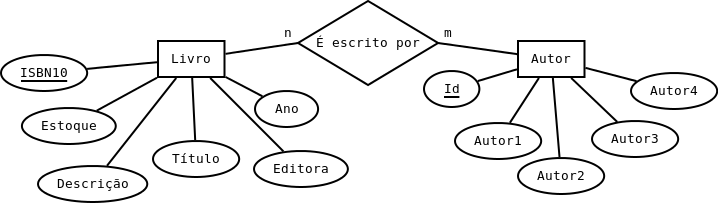
\includegraphics[width=\textwidth]{Imagens/mer.png}
\end{figure}

Como foi dito anteriormente, o servidor é o processo responsável pelo tratamento dos dados, logo (como já era de se esperar) é o processo aonde está o banco de dados e o processo que manipula os acessos ao BD.

	Vale observar que esses tempos foram descontados na hora de fazer a análise do tempo, já que na realidade estávamos interessados em analisar o tempo de transmissão e não o tempo total de execução do processo.

\chapter{Rodando o Servidor em casa}

Como o roteador usa NAT para distribuir o mesmo IP para varios computadores, foi utilizado o recurso de \textit{Virtual Address} para atribuir uma conexão externa a uma porta específica, no caso \textbf{8888}, para um computador com IP específico na rede interna. Como visto na Figura 1.
\begin{figure}[h!]
	\caption{Acessando as configurações do roteador para configurar conexões externas}
%  \centering
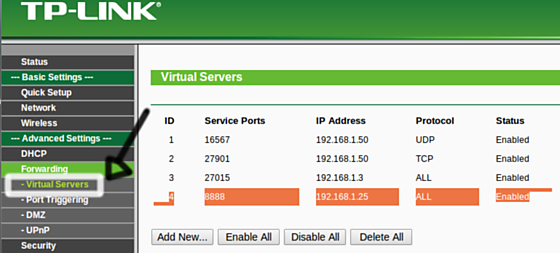
\includegraphics[width=\textwidth]{Imagens/u02.png}
\end{figure}
\\
Após configurar o NAT, foi fixado o IP laptop que sera o servidor, via seu MAC Address, ja que o DHCP gera dinamicamente IP internos à rede. Como visto na Figura 2.
\begin{figure}[h!]
	\caption{Fixando o IP interno do servidor}
%  \centering
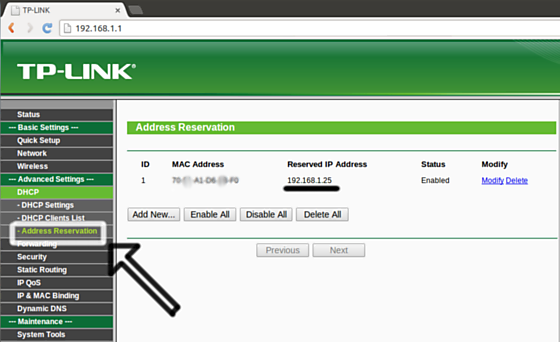
\includegraphics[width=\textwidth]{Imagens/u01.png}
\end{figure}
\newpage
Como o IP provido pela NET Virtua é dinâmico, fez-se um programa em Python apenas para mandar e-mails para a dupla a fim de saber o atual IP da máquina.
\\
Código em Python:
\begin{lstlisting}[language=Python]
import smtplib
import time
import subprocess

while 1:

	# Encontrando o IP externo atraves de uma resposta do icanhazip.com
        ip = subprocess.check_output(['curl', '-s', 'icanhazip.com'])
        
        # Formatando saida do site
        ip = ip.strip()
        ip = ip.decode("utf-8")
        print(ip)

        fromaddr = 'guilhermeag@bol.com.br'
        toaddrs  = 'gagallo7@gmail.com'
        addr2 = 'andrentaz@gmail.com'
        msg = 'IP do laptop: '+ip

        print(msg)

# Credentials (if needed)
        username = 'guilhermeag'
        password = 'segredo'

# The actual mail send
		# Servidor do e-mail e o BOL
        server = smtplib.SMTP('smtp.bol.com.br:587')
        server.starttls()
        server.login(username,password)
        server.sendmail(fromaddr, toaddrs, msg)
        server.sendmail(fromaddr, addr2, msg)
        server.quit()

        time.sleep(120) #espera 2 minutos
\end{lstlisting}

\chapter{Análise de Dados}
Utilizando os arquivos \textbf{.csv} criados pela rotina \emph{logger}, foi possível montarmos tabelas que continham os dados da transmissão.

	Foi calculada a média de tempos de transferência de 119 operações para cada tipo de operação, bem como seu desvio padrão, obtendo assim o respectivo erro.
	
\section{Servidor e Cliente na mesma máquina}	
	Primeiramente, calculamos o tempo de transmissão entre processos rodandos na mesma máquina, ou seja, o processo cliente rodava no host. Isso servirá para comparar o atraso que a rede está dando para a comunicação. A tabela com os tempos de transmissão, computação no servidor e números de recv() estão representadas abaixo:

\begin{figure}[h!]
\caption{Dados da Transmissão em todas as operações numa mesma Máquina}
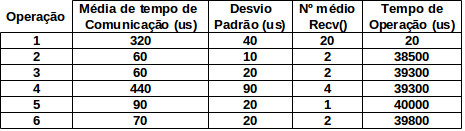
\includegraphics[width=\textwidth]{Imagens/t01.png}
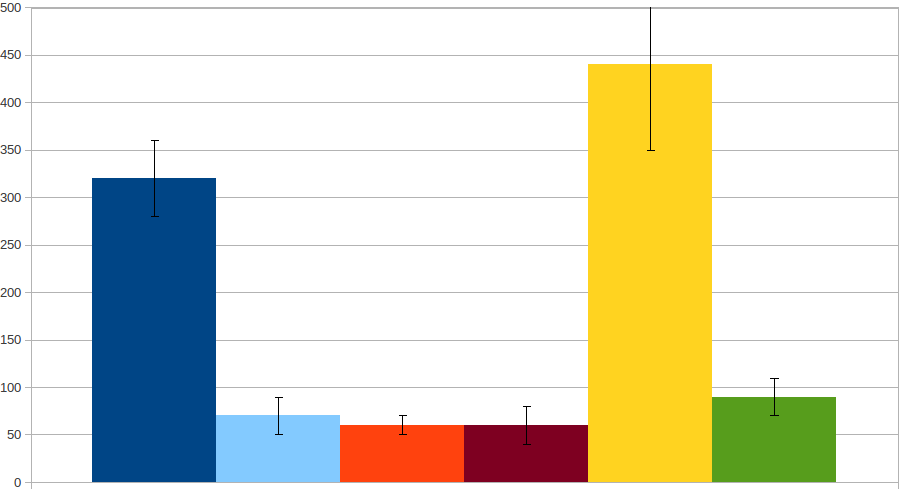
\includegraphics[width=\textwidth]{Imagens/g01.png}
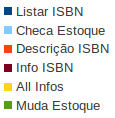
\includegraphics{Imagens/g011.png}
\caption{Gráfico Operação x Tempo Médio de Comunicação}
\end{figure}

Como se pode perceber, a operação que mais demora em tempo de \textit{comunicação} na média é a 4, a qual envia mais bytes. Sendo seguida da 1, que tem mesmo princípio, só que envia menos bytes que a primeira.
Os tempos de \textit{operação} de 2 e 3 são maiores, porque o SQLite3 tem que fazer a busca no banco de dados, o qual está armazenado no HD do servidor. Na verdade, o fator mais importante para a lentidão é que o servidor espera para receber o valor do ISBN nestes dois casos.

Como explicado anteriormente, esses dados foram retirados da situação aonde ambos os processos estão rodando na mesma máquina host. Pelo gráfico, podemos observar que como esperado, a operação mais custosa a nível de tempo é a de enviar todas as informações a respeito de todos os livros para o cliente (barra amarela).

	Entretanto não podemos dizer que o tamanho da mensagem na hora do envio é o único fator de peso na hora de se determinar o tempo necessário para o mesmo. Observando por exemplo a operação de Listar todos os ISBNs e seus respectivos Títulos (barra azul escura), vemos um grande aumento no tempo de transmissão. No caso, o total de dados enviado pelo servidor nesse tipo de operação nem se compara ao tamanho da mensagem em casos como o da operação que envia a descrição de uma dado ISBN (barra laranja). Por exemplo, para o livro “Dom Casmurro”, a descrição do livro supera em muito o tamanho da mensagem enviada para o cliente quando os ISBNs estão sendo listados.
	
	Contudo, a resposta para essa grande quantidade de tempo gasta também pode ser facilmente encontrada se analisarmos outro dado nas tabelas. Podemos ver que para as duas operações mais custosas, a quantidade de procedimentos recv() chamados foi esmagadoramente maior, ou seja, uma grande quantidade de mensagens foi enviada! Isso com certeza é um fator determinante no tempo.
	
	Apesar dessa análise (com processos rodando na mesma máquina) ser de boa ajuda para compreender como funciona o envio de dados, devemos fazer uma análise mais complexa, para um caso real, onde os processos client e server rodam em máquinas diferentes.
	
\newpage
\section{Servidor numa rede e Cliente na outra}
Para isso, o processo server foi executado no notebook do aluno Guilherme Alcarde Gallo, enquanto que o processo client teve sua execução na máquina de nome 'costa', da sala 301, IC03.  Vale notar que neste caso, os além de rodar em máquinas diferentes, os processos rodavam em máquinas que estavam em redes completamente distintas. Isso contribuiu de forma significativa para os tempos de transmissão medidos,  conforme podemos ver nas tabelas e gráficos abaixo, montados com os programas Calc e Writer do Libre Office:

Os resultados a seguir foram obtidos quando o servidor estava localizado na rede Eduroam e o Cliente na rede do Instituto de Computação:

\begin{figure}[h!]
\caption{Dados da Transmissão em todas as operações em redes diferentes}
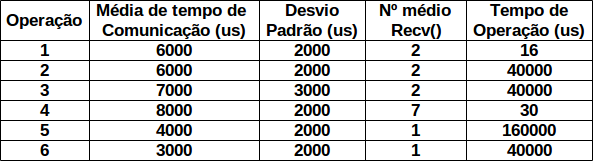
\includegraphics[width=\textwidth]{Imagens/t02.png}
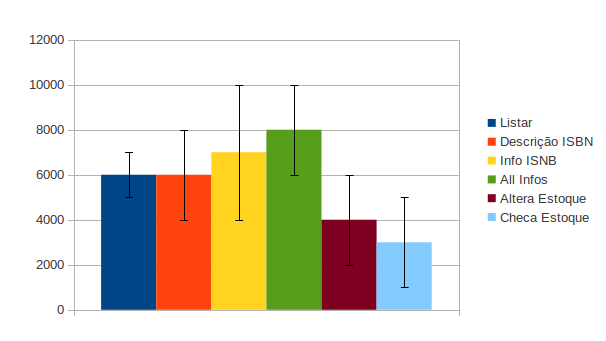
\includegraphics[width=\textwidth]{Imagens/g02.png}
\caption{Gráfico Operação x Tempo Médio de Comunicação}
\end{figure}

Neste caso, podemos observar que os tempos para quase todas as operações (apesar de suas barras de erros) são muito semelhantes. De fato, se considerarmos os erros, podemos dizer que são quase iguais.

	Novamente, se observarmos a tabela correspondente ao gráfico (Figura 5.3), podemos ver que diferentemente da tabela anterior, as duas operações mais discrepantes (Listar ISBN e Todas as Informações) enviam um número de mensagens semelhante ao enviado pelas outras mensagens.
	
	Nesse caso, a operação mais custosa se manteve como a que Lista todas as Informações (o que era de se esperar, já que está operação é a que envia a maior quantidade de dados indiscutivelmente), entretanto, a diferença para a segunda operação mais custosa (nesse caso, a que devolve as informações de um dado ISBN) é de apenas 1000 us.
	
	Cabe notar algo interessante aqui: quando os processos rodaram no mesmo host, o tempo para listar as informações de um determinado ISBN era aproximadamente 18,75\% do tempo para listar todos os ISBNs e seus Títulos, mesmo que na grande maioria das vezes a mensagem enviada para listar a informação seja muito maior do que a da outra operação.
	
	Agora que as máquinas rodam em dois hosts diferentes, podemos notar que não só a situação se inverteu como a operação mais barata (enviar ISBNs e seus Títulos) consome um tempo equivalente a 85,71\% do tempo de Listar as Informações de um dado ISBN. Ou seja, ambos os tempos estão muito próximos.
	
\chapter{Conclusão}
Como observado na parte da análise, existem muitos fatores que determinam os tempos de envio das mensagens através de um protocólo TCP.

	Primeira e obviamente, a rede pela qual a mensagem trafega. Quando executamos os processos em duas máquinas diferentes, os tempos subiram de 440 us para 8000 us (para o processo mais lento), ou seja, quase 20 vezes mais lento! Isso era de se esperar, já que os processos não só estavam em máquinas diferentes, mas em redes diferentes.
	
	Em segundo lugar, o tamanho da mensagem! Tanto para processos rodando num mesmo host, quanto para processos executados em hosts separados, foi possível observar que a operação que mais consumiu tempo foi a que enviava a maior mensagem.
	
	Por fim, tão determinante quanto, a quantidade de mensagens enviada. No caso desse projeto, podemos dizer que esse foi o fator determinante para se determinar qual seria a operação mais custosa.
	
	Apesar dos tamanhos das mensagens serem importantes, como estamos enviando os dados através do protocolo TCP (um protocolo confiável) cada mensagem enviada recebia um tratamento de checagem de erro e de ordem de envio. Ou seja, como no caso dos hosts serem os mesmos, a mensagem foi quebrada em 20 diferentes chamadas de recv(), isso significou que esse protocólo de checagem foi feito muito mais vezes do que no caso de outras mensagens que foram enviadas com apenas 1 único recv().
	
	Talvez, quando realizarmos o projeto utilizando um protocólo de transporte como o UDP, esse fator não seja mais o determinante, já que nesse caso, as mensagens não recebem essa checagem a nível de transporte, sendo que ela deve ser implementada a nível de aplicação.
	
Na prática, percebe-se que o protocolo TCP faz o que promete: mantém uma conexão entre 2 computadores e não deixa nenhuma mensagem se perder. Tanto que a função de read/write ou receive/send só se preocupa em cortar o buffer e saber se enviou/leu tudo o que lhe foi requisitado.

A alta compatibilidade do Unix com este tipo de protocolo também foi muito importante, visto que não houveram problemas com a parte da conexão TCP.

A facilidade de uso do SQLite3 também deve ser citada. Pode salvar muito tempo de trabalho se comparado a fazer um banco de dados em arquivo para um projeto desse porte.

Um fato curioso foi que podemos usar o sistema servidor-cliente e até protocolos de rede para fazer comunicação interprocessos. Apesar de não ser a proposta principal, o sistema na mesma máquina funcionou bem.

\chapter{Referências Bibliográficas}
"Beej's Guide to Network Programming". <http://beej.us/guide/bgnet/>. (Acesso em: 04 abril 2013). \\
"SQLite Documents". <http://www.sqlite.org/docs.html>. (Acesso em: 03 abril 2013).

\end{document}